% question 3
\section{Question 3}
\paragraph{(a)} Dynamic model is given by
\begin{align*}
I_1 \ddot{\theta}_1 &= \tau - K(\theta_1 - \theta_2) - D(\dot{\theta}_1 - \dot{\theta}_2), 
\\
I_2 \ddot{\theta}_2 &= K(\theta_1 - \theta_2) + D(\dot{\theta}_1 - \dot{\theta}_2), 
\end{align*}
\noindent where $K$ is stiffness and $D$ is damping.


\paragraph{(b)} Transfer functions are:
\begin{align*}
G_1(s) &=\frac{\theta_1(s)}{\tau(s)} = \frac{I_2 s^2 + Ds + k}{I_1 I_2 s^4 + s^3(I_1 D + I_2 D) + s^2 (I_1 K + I_2 K) }, \\ 
G_2(s) &=\frac{\theta_2(s)}{\tau(s)} = \frac{Ds + k}{I_1 I_2 s^4 + s^3(I_1 D + I_2 D) + s^2 (I_1 K + I_2 K) }.
\end{align*}


\paragraph{(c)} Figure \ref{fig:q3_OL} describes time-response of open-loop systems ($G_1(s)$ and $G_2(s)$) for different values of stiffness ($K=10[1, 1.4, 1.8, 2.2, 2.6, 3]$ $\mathrm{\frac{N.m}{rad}}$) and damping ($D=1000[1, 1.8, 2.6, 3.4, 4.2, 5]$ $\mathrm{\frac{N.m.s}{rad}}$).

\begin{figure}[h!]
\centering
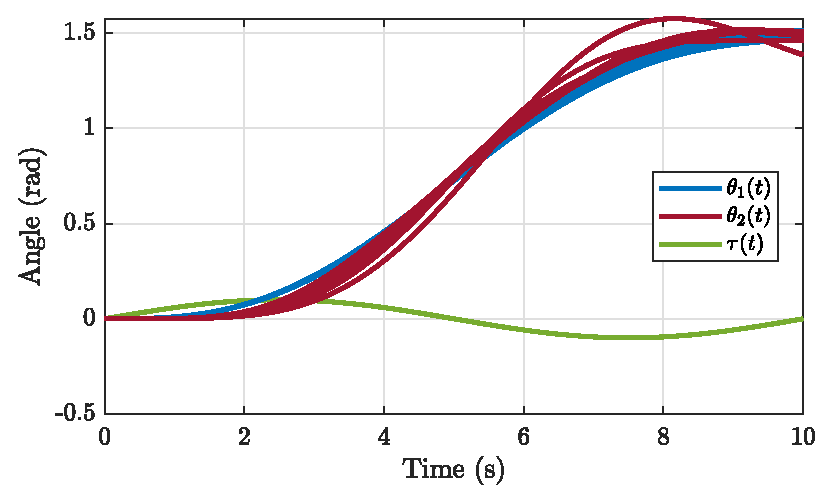
\includegraphics{images/question3/q3_OL.eps}
\caption{Time-response of open-loop systems ($G_1(s)$ and $G_2(s)$) considering sinusoidal input ($\tau=0.1\sin{0.2\pi t}$) and different values of stiffness and damping ($K=10[1, 1.4, 1.8, 2.2, 2.6, 3]$ $\mathrm{\frac{N.m}{rad}}$ and $D=1000[1, 1.8, 2.6, 3.4, 4.2, 5]$ $\mathrm{\frac{N.m.s}{rad}}$). }
\label{fig:q3_OL}
\end{figure}


\paragraph{(d)} On one hand, Figure \ref{fig:q3_rlocus_K_CL} describes root-locus of close-loop system with proportional gain. In this figure, third and fourth poles ($p_3, p_4$) are located in the right half-plane for any proportional gain value. On the other hand, Figure \ref{fig:q3_bode_K_OL} describes bode diagram of open-loop system ($G_2(s)$). In this figure, gain margin is $G_m=-13$ dB and phase margin is $P_m=179^{°}$. Likewise, phase diagram is below $-180^{\circ}$, thus gain margin will be negative for any proportional gain value. In conclusion, both root-locus and frequency response method indicates that close-loop system cannot be controlled with just a proportional gain.


\begin{figure}[h!]
\centering
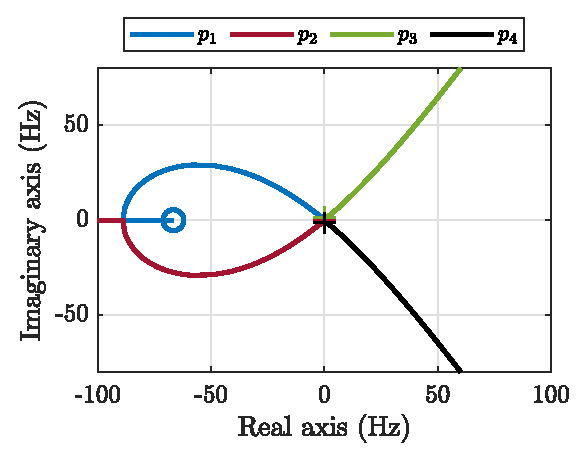
\includegraphics{images/question3/q3_rlocus_K_CL.eps}
\caption{Root-Locus of close-loop system with proportional gain.}
\label{fig:q3_rlocus_K_CL}
\end{figure}


\begin{figure}[h!]
\centering
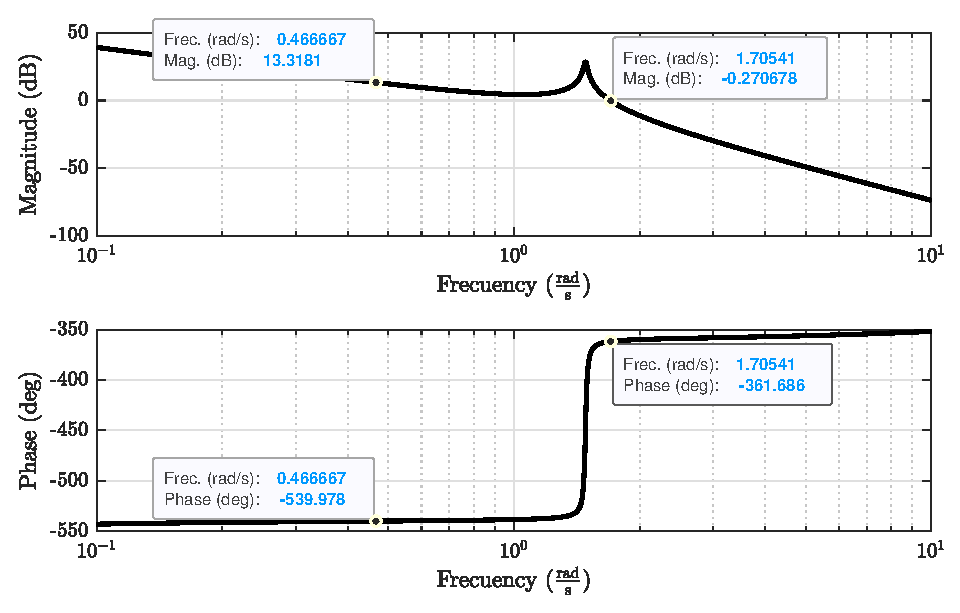
\includegraphics{images/question3/q3_bode_K_OL.eps}
\caption{Frequency response of open-loop system $G_2(s)=\frac{\theta_2(s)}{\tau(s)}$.}
\label{fig:q3_bode_K_OL}
\end{figure}









